\chapter{Ergebnisse}

\begin{comment}

Gliederung meiner Streckenbeschreibung (Yves)

* Übersicht
  * Umfeld des Bauprojekts
  * von wo nach wo
  * historische Einordnung

* konkrter Streckenverlauf
* detalierte Daten (weichen etc ..)


* Probleme
  * bautechnisch
  * gesellschaftlich

* Zeitplan

* Kosten
\end{comment}



\section{Berlin}
\subsection*{Lückenschluss der U5}

Die U-Bahnlinie 5 fährt auf dem Abschnitt zwischen Alexanderplatz und
Friedrichsfelde schon seit 1930 \cite{bkhU5}. Schon im Vorfeld der Eröffnung
dieses Abschnittes, in den 20er Jahren, gab es Planungen, die Linie Richtung
Westen weiter zu verlängern \cite{bvgWebsiteU5}. Ein Vorgriff darauf war die
Eröffnung des Teilstücks U55 zwischen Brandenburger Tor (ehemals Unter den
Linden) und Hauptbahnhof. Die Schaffung dieser Insellösung wurde nötig durch
Verträge zwischen dem Land Berlin und dem Bund anlässlich der Verlegung des
Regierungssitzes \cite{hauptstadtvertrag}. Um die entstande Lücke zu schließen,
plant und baut die BVG eine Neubaustrecke zwischen Alexanderplatz und
Brandenburger Tor. Die ersten Bauarbeiten wurden 2010 begonnen, mit dem
Abschluss wird bisher 2019 gerechnet \cite{bvgWebsiteU5plan}. In unserer Arbeit
widmen wir uns auch der Untersuchung dieser Strecke.

Die neue Strecke beginnt am Alexanderplatz und verläuft vor dem Berliner
Rathaus, um dort auch schon die erste Station Berliner Rathaus zu erreichen
\cite{bkhU5} \cite{bvgWebsiteU5}. Unmittelbar im Anschluss an den Alexanderplatz
wird ebenfalls eine Gleiswechselanlage errichtet. Im weiteren (ebenfalls
unterirdischen) Streckenverlauf wird die Spree von der Station Museumsinsel
unterquert. Ab dort verläuft die Strecke entlang der Straße Unter den Linden, wo
sie im gleichnamigen Kreuzungsbahnhof mit der Linie U6 hält und anschließend, an
der Station Brandeburger Tor, in die bestehende Strecke der U55 mündet. Die
Gesamtläng der Strecke beträgt damit etwa 2,2\,km.

Der Bau wird komplett im Schildvortrieb ausgeführt, was durch den Sandboden vor
Ort erschwert wird \cite{bkhU5}. Desweiteren liegt die Strecke, mit bis zu 25 m unter der Oberfläche,
vergleichsweise tief. Dies wird nötig, da sowohl die Spree als auch die U6
unterquert werden müssen. Ersteres erfordert auch die Konstruktion des Bahnhofs
Museumsinsel im bergmännischen Verfahren, während die anderen Bahnhöfe im
Schachtverfahren gebaut werden können. Neben den baulichen Schwierigkeiten ist
auch der Nutzen des Projektes umstritten \cite{ftdU5}, da die Strecke weitgehend
parallel zu Stadtbahn verläuft und der Kosten-Nutzen-Faktor selbst mit einer geplanten Verlängerung bis Turmstraße
nur knapp über 1 liegt. Insgesamt werden die Kosten für die Strecke auf 435
Mio. Euro geschätzt \cite{bwwwU5}. Wobei sich zu dieser offiziellen Schätzung
auch kritische Kommentare finden, die von noch deutlich höhren Kosten ausgehen
\cite{ftdU5}.

\subsection*{Straßenbahn zum Hauptbahnhof}

In Berlin sind knapp 190\,km Straßenbahnstrecke vorhanden. Die Strecke
der M10 wird dabei von den Überresten eines ehemaligen Ost-West-Ringes
gebildet. Die M10 war seit ihrer Inbetriebnahme für eine reasche
Erweiterung vorgesehen, so dass beide Endhaltstellen als
Stumpfendhaltestellen gebaut wurden. Seit der Eröffnung des
Hauptbahnhofs, im Jahre 2006, sollte die M10 diesen eigentlich schon anfahren. Die Strecke soll vom Nordbahnhof über die
Invalidenstraße bis zum Hauptbahnhof verlängert
werden \cite{tsM10}.

Der neue, 2.4\,km lange zweigleisige Abschnitt der Strecke verläuft vom
Nordbahnhof die Invalidenstraße entlang, vorbei an der Humbold
Universiätt und am Invalidenpark, bis zum Europaplatz vor dem
Hauptbahnhof \cite{M10bInfo}. Entlang dieser Strecke entstehen
drei neuen Haltestellen pro Fahrtrichtung. Diese Haltestellen werden
mittels Haltestelleninsel und Haltestellenkap realisiert. Hinter dem
Hauptbahnhof wird die Strecke, mit einer 1.1km langen einspurigen
Wendeschleife mit 3 zusätzlichen Haltestellen, abgeschlossen
\cite{zdfM10}. Während den Baumaßnahmen wird die Invalidenstraße
4-spurig ausgebaut. Die beiden mittleren Spuren werden dann zusammen
vom Autoverkehr und den Straßenbahnen benutzt
\cite{flyerInvalidestr}. Laut ersten Planungen soll das gesamte
Projekt 22.8\,Mio.\,Euro kosten und schon 2014 sollen die ersten
Bahnen die Strecke befahren \cite{mopoM10}.


Während der Bauarbeiten werden auch Tiefbauarbeiten von mehreren
Energieversorgern und Telekomunikationsunternemen
durchgeführt. Außerdem wir der U-Bahntunnel neu abgedichtet und
der vorhandene Durchlass für die Panke
erneuert \cite{flyerInvalidestr}. Diese umfangreichen Baumaßnahmen
wurden in der ersten Planungsphase nicht beachtet, da der zuständige
Senator von der Stadtentwicklungsbehörde die Straßenbahn schnell bauen
wollte. Dies führte allerdings zu erheblichen Verzögerungen, da die
gesamte Planung erneut aufgerollt werden
musste \cite{bzSchnell}. Außerdem gibt es viele Stimmen die der Meinung
sind, der geplante Ausbau der Invalidenstraße führe dazu, dass die
Straßenbahn massiv durch den Autoverkehr behindert wird. Dadurch ist
die Fahrzeit der Tram nicht wesentlich geringer als die Fahrzeit der
Busse auf der gleichen Strecke und der Nutzen der Neubaustrecke ist
geringer als geplant \cite{protram}.

\section{Hamburg}
\subsection*{U4}

Die U4 in Hamburg ist eine 2012 neugeschaffene Linie, die sich allerdings die
meisten ihrer Haltstellen mit der U2 teilt. Ihre Aufgabe ist der Anchluss der
Hafencity an das Hamburger Hochbahnnetz \cite{keuHH}. Um dies umzusetzen, wurde
abzweigend von der vorhanden U2-Station Jungfernstieg, eine neue Strecke gebaut,
die im Rahmen dieser Arbeit ebenfalls untersucht wird. Dabei werden wir uns vor
allem auf den schon fertigen Abschnitt konzentieren. Die im Bau befindliche
Verlängerung bleibt außen vor.

Die Neubaustrecke hat eine Gesamtlänge von ca. 4\,km \cite{keuHH}. Sie verläuft
von Jungfernstieg ausgehend unter der U3 hindurch, um dann anschließend das
Hafenbecken zu unterqueren. Ihre beiden Haltestellen Überseequartier und
HafenCity Universität liegen dann beide auf dem Gebiet der Hafencity. Beide
Tunnelstationen konnten in offener Bausweise errichtet werden. Alle anderen
Streckenteile verlaufen ebenfalls unterirdisch und wurden im
Schildvortriebverfahren gebaut.

Neben den bautechnischen Schwierigkeiten der Hafenunterquerung hat auch dieses
Projekt mit Kritik auf verkehrspolitscher Ebene zu kämpfen. So wird die
unterirdische Streckenführung kritisiert, da sie teurer sei, als eine
Hochbahnlösung. \cite{hamburgerAbendblattu4}.

\section{Stuttgart}

Die Geschichte der Stuttgarter Straßenbahn geht zurück bis ins Jahr 1868. In den
1960er- und 1970er-Jahren wurden die damals oberirdisch liegenden
Streckenabschnitte im Innenstadtbereich unter die Erde verlegt. In den
1970er-Jahren gab es Planungen zum Aufbau eines separaten U-Bahn-Netzes, es wurde sich
jedoch dafür entschieden, das (meterspurige) Straßenbahnnetz sukzessive zur
(normalspurigen) Stadtbahn umzubauen. Im Jahr 1985 wurde die erste
Stadtbahnlinie am südlichen Stadtrand eröffnet, Ende 2007 wurde der Betrieb auf
der Meterspur eingestellt \cite{SSBgeschichte}.

Die im Folgenden vorgestellten Strecken der Linie U15 sind Teil dieses Umbaus.

\subsection*{U15 nach Ruhbank}

Als letzte \cite{u15vorinfo} Linie wurde die Straßenbahnlinie 15 durch die
Stadtbahnlinie U15 ersetzt. Die, gemeinsam mit anderen Linien befahrenen,
Streckenteile wurden schon im Zuge des Umbaus der anderen Linien, zu einem
Dreischienengleis ausgebaut \cite{beob}, um dort in der Zwischenphase mit beiden
Zugtypen fahren zu können. Daher fehlte nur noch der Umbau der südlichen
Strecke zwischen Olgaeck und Ruhbank, ein kurzes nur von der Linie 15 befahrenes
Stück nördlich des Hauptbahnhofs sowie das nördliche Ende der Linie zwischen
Zuffenhausen und Stammheim \cite{u15mail}. Die Strecke nach Ruhbank wird im
Folgenden untersucht, die Strecke nach Stammheim im darauffolgenden Abschnitt.

Der Umbau der Strecke nach Ruhbank erfolgte zwischen 2005 und 2007 unter
laufendem Betrieb \cite{u15seb}. Im größten Teil der Strecke wurde der
Streckenverlauf beibehalten, nur im südlichsten Abschnitt, wo die alte Strecke
auf etwa 1\,km, etwas abseits der Straße, im Wald verlief, wurde die
Stadtbahnstrecke näher an die Straße gelegt.

Dennoch vermuten wir, dass die Kosten des Projekts ungefähr denen eines
kompletten Neubaus entsprechen. Dafür spricht, dass vielfach der Straßenraum
neu geordnet wurde (insbesondere aufgrund der nun nötigen Hochbahnsteige und
ihrer Zugänge), auf ca. 70 Metern Länge eine Sondergründung notwendig war
\cite{u15mail} und davon ausgegangen werden kann, dass die alten Materialien
(Gleise etc.) nicht wieder verwendet wurden. In wie weit durch Verwendung
existierender Infrastruktur wie Gleisunterbau und Stromversorgung Einsparungen
erzielt wurden, ist uns nicht bekannt. Möglich ist jedoch, dass bei einem
kompletten Neubau eine Verbreiterung der Straße mit beispielsweise Abriss von
Häusern nötig geworden wäre.  Andererseits ist davon auszugehen, dass der Umbau
bei laufendem Straßenbahnbetrieb den Bau stark verteuert hat.

Die Strecke zweigt an der, nahe der Innenstadt und noch fast auf Höhe des
Talkessels (264\,m) liegenden, Haltestelle „Olgaeck“ ab und führt in 4,9\,km
zur, Nahe des Fernsehturms, auf 476\,m gelegenen Haltestelle „Ruhbank“
\cite{u15vorinfo}. Dies ergibt eine durchschnittliche Steigung von 4,2\,\%,
die maximale Steigung der Strecke beträgt 8,5\,\%. Die bis dato höchste
Steigung im Netz betrug 7\,\%, was besondere Tests nötig machte, die von den
speziell für Stuttgart konstruierten Fahrzeugen jedoch erfolgreich bestanden
wurde \cite{u15vorinfo}. Von den 4,9\,km sind 2,1\,km straßenbündig
angelegt, in diesem Bereich beträgt die Höchstgeschwindigkeit 50\,km/h, sonst
60\,km/h.

Es gibt entlang der Strecke 8 Haltestellen \cite{u15splan} (die am unteren Ende
der Neubaustrecke liegende Haltestelle Olgaeck wurde nicht mitgezählt, da sie
noch im Bereich der vorher umgebauten Strecke liegt). Die Strecke enthält 12
Weichen.

Geplant wurde vor Baubeginn mit Kosten von \EUR{46 Mio}. \cite{u15vorinfo},
letztlich kostete das Projekt \EUR{48 Mio}. \cite{u15seb}.

\subsection*{U15 nach Stammheim}

Nach der Eröffnung der Strecke nach Ruhbank wurde zum Fahrplanwechsel im
Dezember 2007 die Straßenbahnlinie 15 vollständig eingestellt und auf dem
nördlichen Streckenast zwischen Zuffenhausen und Stammheim ein Busersatzverkehr
eingerichtet \cite{u15sv}.  Im Frühjahr 2008 begannen die Bauarbeiten
\cite{u15seb}, eröffnet wurde die Strecke im Dezember 2011 \cite{u15sv}.

Wie bei der südlichen Umbaustrecke der U15 gehen wir davon aus, dass sich die
Kosten kaum von denen einer Neubaustrecke unterscheiden. Zu den oben genannten
Argumenten kommt hier noch noch die Tatsache, dass die Strecke auf gut einem
Kilometer Länge in einen Tunnel verlegt wurde.

\begin{wrapfigure}{r}{.51\textwidth}
  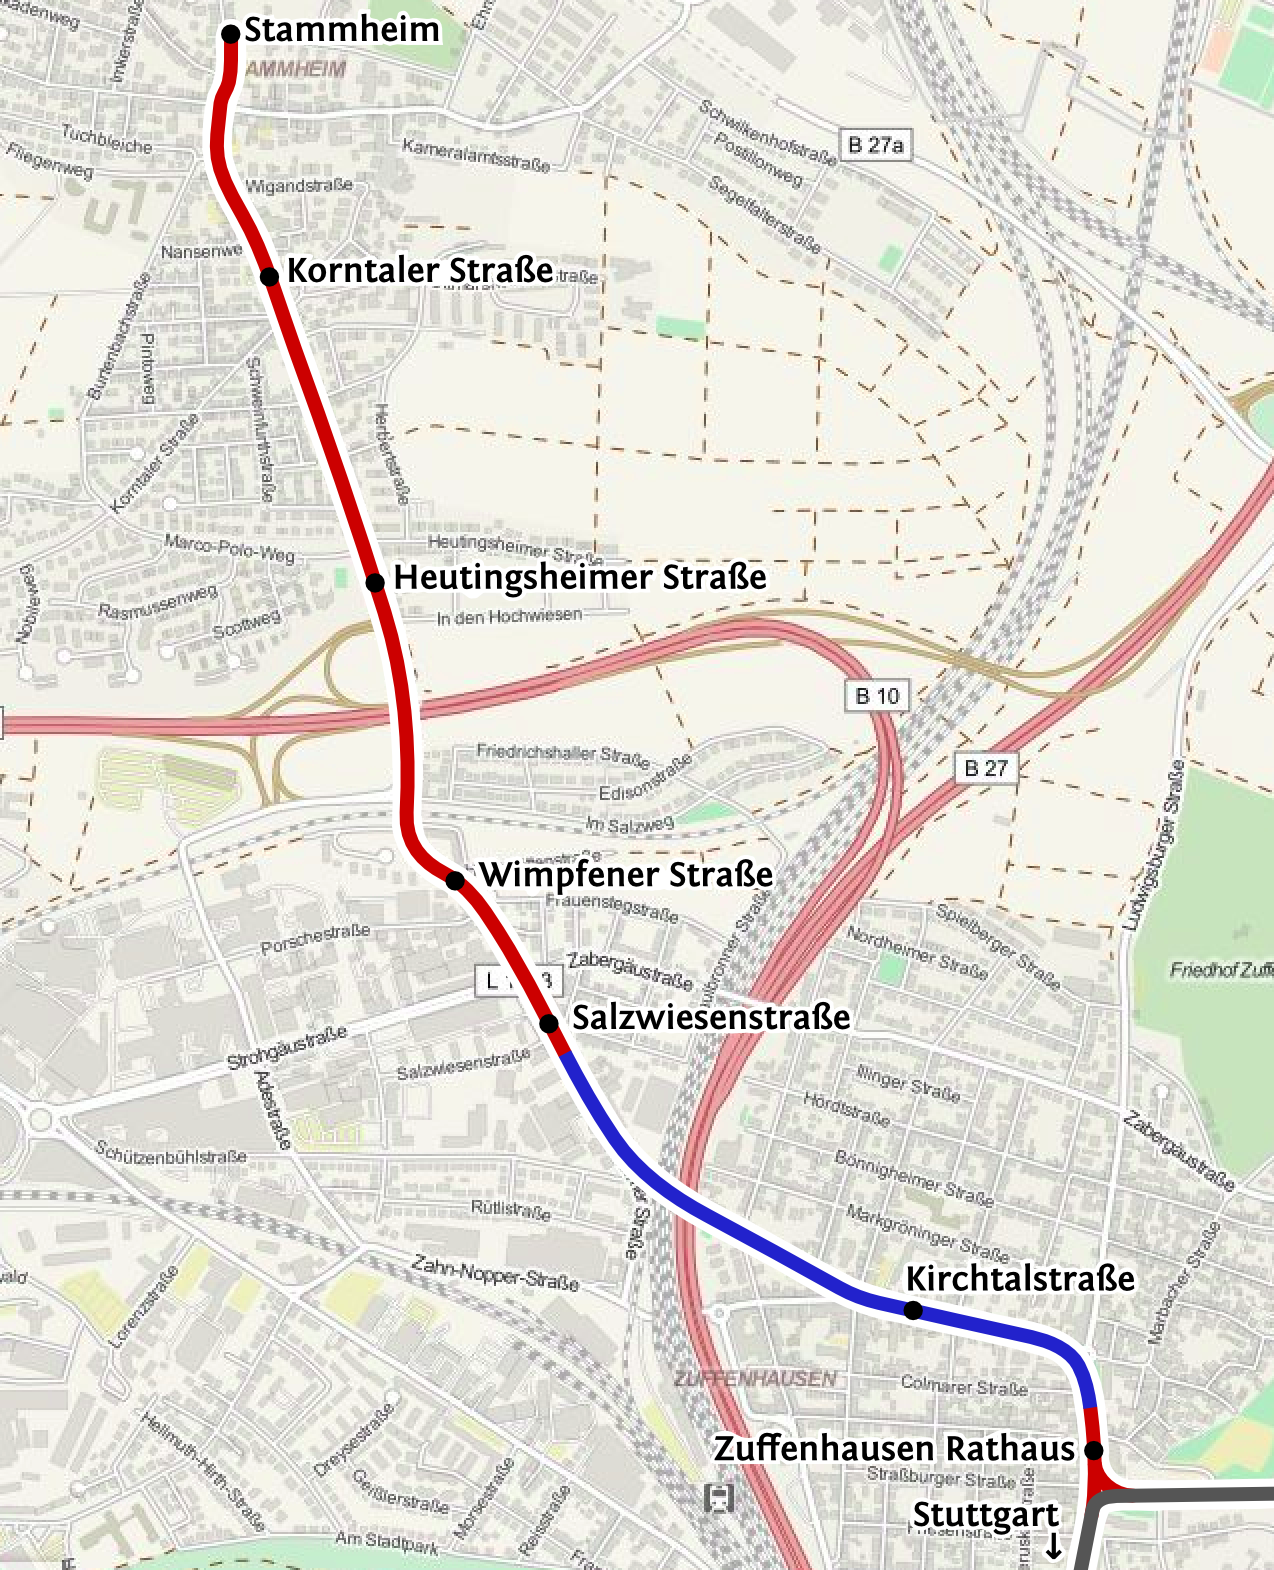
\includegraphics[width=.5\textwidth]{maps/Stuttgart.png}
  \caption{Strecke nach Stammheim}
\end{wrapfigure}

Die Strecke zweigt in Zuffenhausen von einer anderen Linie ab. Direkt dort liegt die erste Haltestelle, die zugleich die Tunnelrampe bildet. Im ersten Abschnitt (Länge: 580\,m), in der Einkaufsstraße des Stadtteils, wurde dieser in offener Bauweise errichtet.
Danach kürzt die Strecke den Verlauf der Straßenbahn durch eine kleinere Straße ab. An deren Ende unterquert der Tunnel eine Bundesstraße und eine Bahnlinie und endet wieder im Bereich einer Haltestelle. In diesen beiden Abschnitten wurde der Tunnel bergmännisch gebaut (Länge: 480\,m) \cite{u15mail} \cite{u15sv} \cite{u15nplan}.
Weiter verläuft die Strecke wieder entlang der alten Führung der Straßenbahn, innerhalb der Bebauung von Zuffenhausen bzw. Stammheim größtenteils auf der Straße, auf einem etwa 500\,m langen Abschnitt dazwischen auf einem eigenen Gleiskörper zwischen den Fahrbahnen \cite{u15nplan} bis zur Endhaltestelle, für die eine Gebäudereihe abgerissen werden musste \cite{u15sv}.

Die Strecke ist 3,0\,km lang, davon sind insgesamt 0,8\,km straßenbündig und 1,06\,km in einem Tunnel.
Im oberirdischen Abschnitt beträgt die Höchst\-ge\-schwin\-dig\-keit 50\,km/h, im Tunnel 70\,km/h.
Entlang der Strecke gibt es sechs Weichen \cite{u15mail}.

Trotz des Tunnelanteils haben wir die Strecke als Tramstrecke kategorisiert, da sie überwiegend oberirdisch verläuft. Die Kosten liegen jedoch erwartungsgemäß weit über denen der anderen Tramstrecken.

\section{Magdeburg}

Seit 2000 wird in Magdeburg eine zweite Nord-Süd-Verbindung
gebaut. Bis zum Jahre 2019 soll das Straßenbahnnetz in 7
Bauabschnitten um 13.5\,km erweitert und damit die Grundlage
für die Weiterentwicklung der Landeshauptstadt geschaffen
werden. \cite{mvbNordSued}

\begin{figure}[h]
  \begin{center}
    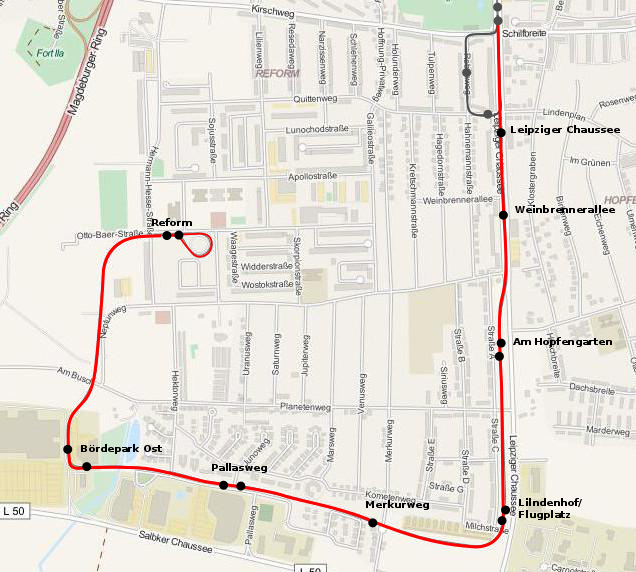
\includegraphics[width=0.8\textwidth]{maps/Magdeburg.png}
    \caption{Verlauf der Strecke nach \textit{Reform}}
  \end{center}
\end{figure}

Hier beschäftigen wir uns nur mit dem 3. Bauabschnitt, der Strecke
über den \textit{Bördepark} nach \textit{Reform}. Die 3.6\,km lange
Strecke beginnt in der Leipziger Chaussee und verkürzt die bisherige
Fahrzeit mit dem öffentlichen Nahverkehr um 14\,min auf 10\,min. Die
komplette Strecke ist zweigleisig ausgelegt und endet mit einer
Wendeschleife. Nur etwa 500\,m verlaufen in der Mitte der Leipziger
Chaussee. Die restliche Strecke wurde als eigener Gleiskörper
ausgeführt und bedient in beiden Richtungen 8 barrierefreie
Haltestellen. \cite{ba3reform}

Die neue Linie bindet sowohl das Wohngebiet in Reform an, als auch die
großen Einkaufstädten im Bördepark im Süden von Magdeburg. Von den
22.4\,Mio.\,Euro \cite{volksstimme2009} sind gut 80\% (18\,Mio.\,Euro
\cite{ba3reform}) Fördermittel vom Bund und Land. Die Neubaustrecke
nach Reform wurde im Gegensatz zu anderen Abschnitten der neuen
Nord-Süd-Verbindung gut von der Bevölkerung angenommen. Das mag
daran liegen, dass die Strecke nicht durch die Altstadt führt. Bei
einem anderen Bauabschnitt gab es Bürgerproteste, da die Bewohner
befürchteten, dass die neuen Vibrationen der Straßenbahn zu Schäden an
der Gebäudesubstanz führen würden. \cite{volksstimme2008}

\section{Nürnberg}

Am 14. Juni 2008 ging in Nürnberg die vollautomatische U-Bahn Deutschlands ans Netz\cite{nbBr}. Das Besonde: Sie teilt sich einen, sechs Stationen langen, Streckenabschnitt mit der, mittlerweile ebenfalls automatisierten, U2. Wäre der gemeinsame Streckenabschnitt nicht Automatisiert, so wäre der zeitliche minimalabstand, zwischen zwei Zügen, 200\,Sekunden\cite{nbBr}. Das Würde bedeuten, das jede Linie nur alle 6-Minuten verkehren könnte. Durch die, RUBIN ({\bf R}ealisierung einer automatisierten {\bf U}-{\bf B}ahn {\bf i}n {\bf N}ürnberg) genannte, Automatisierung der U2 und U3 ist ein minimaler zeitlicher Abstand von 100\,Sekunden möglich. Dies ermöglicht einen 3-Minuten Takt für beide Linien. Außerdem wurde die Sicherheit verbessert. Sensoren in den Türen sorgen dafür, das keine Menschen eingeklemmt werden und ein Bahnsteigsicherungssystem erkennt, wenn sich Personen im Gleisbett befinden\cite{nbBr}. Die Vorteile liegen auf der Hand und es wird offenbar, das dies mehr ist, als überflüssiges Prestige. 

\begin{figure}[h]
  \begin{center}
    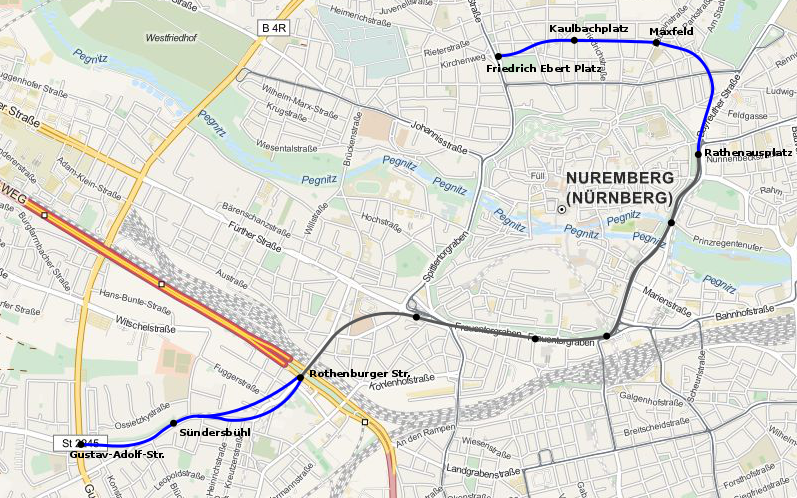
\includegraphics[width=0.8\textwidth]{maps/Nuernberg.png}
    \caption{Streckenverlauf der U-Bahn (Ausbaustufen 1 und 2)}
  \end{center}
\end{figure}

Die erste Ausbaustufe der U3 umfasste zwei Bauabschnitte: Den Bauabschnitt 1.1 im Süden, von der Station Gustav-Adolf-Str. über Südersbühl auf die U2-Station Rothenburgerstr. und der Bauabschnitt 1.2 im Norden, von der U2-Station Rathenausplatz nach Maxfeld. Diese beiden Abschnitte wurde gemeinsam am 14. Juli 2008 in Betrieb genommen. Die zweite Ausbaustufe, der Bauabschnitt 1.3, verlängert die U3 im Norden um zwei Stationen. Die aktuelle Endhaltestelle, seit Dezember 2011, ist der Friedrich-Ebert-Straße. Aktuell wird an der dritten Ausbaustufe gearbeitet, die die U3 um weitere zwei Stationen im Nordwesten verlängern soll. Ihre fertigstellung ist für Ende 2016 geplant\cite{nbNord3}.

Der 1,6\,km lange Bauabschnitt 1.1 hat \EUR{62 Mio} gekostet, der 1,2\,km lange Bauabschnitt 1.2 \EUR{42 Mio} und der 1,1 km lange Bauabschnitt 1.3 \EUR{66 Mio}\cite{nbBr}. Die dritte Ausbaustufe, 1.1\,km lang, wird auf \EUR{83 Mio} geschätzt\cite{nbNord3}. Das sind insgesammt \EUR{253 Mio} für 5\,km Strecke und 7 U-Bahnhöfe. 

Für das RUBIN-System wurden \EUR{112 Mio} ausgegeben, für die Anschaffung von 38 Fahrzeugen \EUR{140 Mio}\cite{nSi}.

Die Planungen für eine Erweiterung der U3 nach Südwest wurden mittlerweile verworfen, da das Kosten-Nutzen-Verhältnis unter eins liegt.

Die U-Bahntunnel wurden in einer Tiefe von 5 bis 10 Metern gebaut und verläuft komplett unter der Erde\cite{nbRef3}. Die Tunnel wurden überwiegend bergmännisch gebaut. Da wo der Tunnel in Schachtbauweise gebaut wurde, etwa an den Stationen und dem Strckenabschnitt, um die Station Kaulbachplatz herum, wurde ein Verfahren benutzt, in dem die Baugrube frühzeitig durch eine Stahlbetongdecke abgedeckt wurde, um die Anwohner zu schonen\cite{nbBr}. 

Als zwischen 1995 und 1999 die Flughafenanbindung der U2 gebaut wurde, haben Inhomogenitäten im Keupersandstein zu schnellen Verkleben des Schneidkopf mit der Gesteinsmasse geführt, und die Vortriebsleistung des Schneidkopfes erheblich verschlechtert\cite{nbGeo}. Auch die U3 führte teilweise durch Keupersandstein\cite{nbRef3}. Das der U-Bahn-Bau in Nürnber mittlerweile kein Neuland mehr ist, kam dem Projekt vermutlich zugute.

\section{Bremen}
\subsection*{Verlängerung der Linie 1}

Die Zeiten in denen in Bremen Straßenbahnlinien durch Busverbindungen ersetzt wurden scheinen entgültig vorbei zu sein. 26 Jahre nach dem die Linie 4 stillgelegt wurde, ging sie im Mai 1998 wieder auf Fahrt \cite{bSv11}. Zwischen 1997 und 2009 hat die Bremer Straßenbahn einen Zuwachs der Fahrgastzahlen von 92,5 Mio auf 101 Mio Fahrgäste verzeichnet \cite{bNp10}. Auch die Linie 6 wurde mittlerweile erweitert und 2006 ging ein neuer Abschnitt der Linie 3, die ``Hafenstraßenbahn'' ans Netz. 

Die derzeit jüngste Erweiterung des Bremer Strßenbahnen-Netzes ist die Verlängerung der Linie 1. Baubeginn des 4,8km langen Abschnitts war der 30. April 2010 \cite{bNp10}. ``Rund 16 000 Einwohner, Kunden der Einkaufsstäten und Freizeitstätten {…} und Arbeitskräfte'', so Georg Drecksler, der Vorstandsvorsitzende der BSAG, werden durch dieses Projekt besser angebunden \cite{bNp10}. Er begreift die neue Linie als Aufwertung für den Stadtteil Osterholz und Standortvorteil für Bremen. Mittlerweile wurde auch der letzte der insgesammt drei Bauabschnitte\cite{bSv12} fertiggestellt. Die Verlängerung der Linie 1 hat die Lücke geschlossen zwischen der bisherigen Endhaltestelle ``Osterholz Schweizer Eck'' und dem 9 Haltestellen entferntliegenden Regionalbahnhof, welcher übrigens auch ein wichtiger Busknotenpunkt ist. Auch der Einkaufsmarkt an der Hans-Bredow-Straße ist nun ans Tramnetz angebunden.

Die Verlängerung ist durchgängig zweigleisig und hat an der Endstation eine Wendeschleife und ein zweites Tramgleis. Sie ist für Einrichtungsfahrzeuge ausgelegt. Über große Teile der Stecke befinden sich die Gleise auf einem eigenen Bahnkörper\cite{bBub11}. 

Der Gesammtpreis des Projektes beträgt \EUR{62 Mio}. Es ist davon auszugehen, das in dieser Summe auch Ausgaben stecken, die nicht in Straßenbahn-Infrastrucktur investiert wurden. Denn das Infrastruckturprojekt umfasste auch den Bau von Rad- und Fußwegen, sowie das Pflanzen von Bäumen\cite{bNp10}. Gebaut wurde außerdem eine Energiespeicher für Bremsenergie\cite{bSv12}. Notwendig, und sicherlich Kostenspielig war auch die Vergrößerung einer Eisenbahnunterführung, damit sich die Straßenbahn auch an dieser Stelle die Fahrbahn nicht mit dem Individualverkehr teilen muss. Eine genauere Aufschlüsselung der Kosten diese Infrastruckturprojektes war in den öffentlichen Quellen leider nicht zu finden. 

Die Straßenbahn-Zukunft in Bremen sieht übrigens weiterhin rosig aus:
In den kommenden Jahren sind fünf weitere Strecken mit einer Gesammtlänge von 25km geplant \cite{bNp10}.


\section{Freiburg}

Die Freiburger Stadtbahn ist das Rückgrat des Personennahverkehrs in der gut 210.000 Einwohner zählenden Stadt. In den vergangenen 20 Jahren gab es eine Reihe von Erweiterungen, zuletzt wurde 2006 die Strecke ins Vauban eröffnet (siehe unten), die Verlängerung in Zähringen soll 2014 eröffnet werden (siehe weiter unten), im Juni 2013 war Baubeginn für eine neue Strecke zur Messe.

\subsection*{Vauban}

Baubeginn für die Strecke war im Herbst 2003, nachdem sie Ende 2005 im wesentlichen fertiggestellt war, ging sie im April 2006 in Betrieb \cite{FRabv}.

Die Strecke zweigt an der Haltestelle \textit{Heinrich-von-Stephan-Straße} von der 2004 eröffneten \textit{Stadtbahn Haslach} ab.
Sie verläuft durchgängig in Straßenmitte auf eigenem, begrünten Bahnkörper, nur auf einem etwa 200 Meter langen Abschnitt nutzt sie die Straße mit, um den Neubau einer hohen Eisenbahnbrücke zu vermeiden.
Nach etwa 1,5\,km wird der Neubaustadtteil Vauban erreicht, der auf einer von Anfang an freigehaltenen Trasse bis zum Ende durchquert wird.
Hier endet die Strecke an einer Wendeschleife; die Möglichkeit eines Weiterbaus wurde vorgesehen.
Außerdem soll hier eine Umsteigemöglichkeit zum Bahnverkehr geschaffen werden, sobald durch den viergleisigen Ausbau der Rheintalbahn auf der Altstrecke genügend Kapazitäten für ein S-Bahn-Netz freigeworden sind \cite{FRabv} \cite{beob}.

Insgesamt ist die Strecke 2,5\,km lang und bedient dabei 5 Haltestellen \cite{FRabv}.
Der Bau kostete \EUR{18,7 Mio} \cite{FRabv2}, vor dem Bau wurde mit etwa \EUR{24 Mio} gerechnet \cite{FRbku}.


\subsection*{Zähringen}

Im Juli 2011 war Baubeginn für die Verlängerung der Stadtbahn über den bisherigen Endpunkt hinaus weiter nach Zähringen hinein, im April 2014 soll die Strecke eröffnet werden. Es wird von Kosten von \EUR{28,3 Mio} ausgegangen \cite{FRabz}.

Die Strecke beginnt an der bisherigen Endhaltestelle \textit{Reutebachgasse}, die im Zuge der Verlängerung etwa 100 Meter nördlich des bisherigen Endpunkts verlegt wird. Bis auf ein etwa 100 Meter langes Teilstück liegt die Strecke vollständig auf einem eigenen, begrünten Gleiskörper. Die letzten beiden Haltestellen liegen außerhalb von bebautem Gebiet, die Strecke endet an der Gemarkungsgrenze mit einer Wendeschleife. In Zukunft soll die Strecke bis in den Nachbarort \textit{Gundelfingen} weitergebaut werden \cite{FRabz}.

Drei Ingenieursbauwerke sind im Verlauf der Strecke nötig: Eine Brücke über einen Bach wird durch einen breiteren Neubau ersetzt, der auch die Stadtbahn aufnehmen kann; es muss eine neue Brücke gebaut werden, unter der die Stadtbahn die Güterbahnstrecke unterquert; außerdem ist eine 100 Meter lange Stützmauer nötig \cite{FRabz}.


\section{Darmstadt}

\subsection*{historisch}

Darmstadt ist eine mittelgroße Stadt in Hessen. Um 1900 lebten rund 70.000
Menschen in Darmstadt. Daher war die Stadt, die zugleich Sitz des Großherzogtums
Hessen-Darmstadt war, bestrebt, eine Straßenbahn einzurichten. Das erste Netz
entstand somit in den Jahren 1897 bis 1903 und verband die Viertel der
wohlhabenden Bevölkerung, die Innenstadt und die Bahnhöfe miteinander. \cite{buernheim1997bahnen}

Zur Inbetriebnahme der Darmstädter Straßenbahn wurden 1897 zwei Strecken
errichtet, welche sich zwischen dem Schloß und dem Pädagog die Strecke
teilten. Die erste Linie verlief von der Station \emph{Böllenfalltor}, an
welcher sich der Betriebshof befand, entlang einer damals nur schwach
besiedelten Villenkollonie über den Friedhof, das Pädagog und das Schloß (wo
Anschluss an drei Vorort-Dampfstraßenbahnlinien bestand) zu den
(Haupt)-Bahnhöfen. Die zweite Linie wurde von der Taunusstraße (Brauereiviertel)
über das Schloß und das Pädagog bis zur Hermannstraße. Letztere Station endete
somit an der Stadtteilgrenze zu einem der wohlhabenderen Darmstädter Vierteln. \cite{hoeltge1992hessen}

In den folgenden Jahren wurden verschiedene Streckenergänzungen vorgenommen. So
wurde 1900 die Strecke zur Hermannstraße bis zur Ludwigshöhstraße verlängert und
ershcloss somit das Viertel Bessungen. 1902 wurde die Strecke zur Taunusstraße
bis zur Fasanerie verlängert und erschloss somit ein Villenviertel und ein
Ausflugsziel. 1903 folgten die Errichtung einer neuen Strecke von den Bahnhöfen
zum Schloßgartenplatz, wodurch das Paulusviertel erschlossen wurde, in welchem
viele Beamte wohnhaft waren. Ebenfalls 1903 wurde eine Strecke vom Schloß in die
südliche Innenstadt errichtet, um eine Konkurrenz zu einer der
Dampfstraßenbahnstrecken aufzubauen.

Die Streckenbauten von 1897 umfassten 6,4 km Strecke, von denen 0,9 km
zweigleisig ausgeführt wurden. Die eingleisigen Streckenabschnitte hatten
insgesamt 8 Ausweichstellen.  Die Baukosten betrugen 287.000 Mark, was
umgerechnet und inflationsbereinigt etwa 5,1 Mio. Euro entspricht. \cite{UmrechnungGoldmark}

Die Streckenaus- und -neubauten von 1899 bis 1903 umfassten insgesamt 5,98 km,
von denen 0,64 km zweigleisig ausgeführt wurden. Es wurden 4 Ausweichstellen
vorgesehen. Die Kosten für die Erweiterung beliefen sich auf 1,2 Mio. Mark,
wobei hierin auch 16 neue Fahrzeugen enthalten sind. Da die 1897 beschafften 18
Fahrzeuge geringerer Länge und einfacherer Technik 262.000 Mark kosteten, was
etwa der Hälfte der Gesamtkosten entspricht, ist davon auszugehen, dass etwa die
Hälfte der Investitionen in den Ausbau auf die Fahrzeugbeschaffung
entfiel. Somit kostete der Ausbau ca. 600.000 Mark. Das entspricht etwa 5,6 Mio.
Euro.

Die Strecken wurden weitestgehend in Straßenlage in einfacher Bauform
ausgeführt. Dabei wurde der Untergrund verdichtet, die Schienen darauf gelegt
(und mittels Querstreben in ihrer Spurweite gefestigt) und wahlweise mit Sand
aufgefüllt oder gepflastert. Die Fahrleitung wurde durch einfache Wandrosetten
an den umliegenden Häusern befestigt, sofern genügend hiervon vorhanden waren.

Bei der Erstausstattung 1897 wurden, abweichend von der vogehend beschriebenen
Standardbauform, 1,64 km als besonderer Bahnkörper ausgeführt und mit
Oberleitungsmasten versehen.  Bei den Ausbauten von 1902 wurden abweichend etwa
1,29 km mit Oberleitungsmasten und Querverspannung ausgeführt.

Aus der Bauphase sind keine Probleme bekannt geworden. Lediglich bei der
Trassierung von 1897 war ein Häuserblock im Weg, welcher abgetragen werden
musste. Über Entschädigungszahlungen ist nichts bekannt, da sich die fragliche
Stelle jedoch in der armen Innenstadt befand ist davon auszugehen, dass keine
Entschädigungszahlungen in nennenswertem Umfang gezahlt wurden.

Der Bau der ersten Strecken erfolgte zwischen April und Novemver 1897.

\subsection*{aktuell}

Darmstadt hat derzeit etwa 140.000 Einwohner. Die Dampfbahnstrecken wurden bis
1926 elektrifiziert. Zudem gab es diverse Streckenneubauten und
-einstellungen. Das Netz umfasste 2009 somit etwa 40 km Länge.

Um die Verkehrssituation im Norden Darmstadts zu verbessern, wurde von Dezember
2006 bis Juni 2009 die Strecke zwischen Merck und Arheilgen gesperrt und
grundlegend saniert \cite{eoDaAr1}.  Bis auf die Trassenführung und die
Haltestellenlage bleib jedoch nichts erhalten, weshalb die Strecke als Neubau
gewertet werden kann. Ab 2009 bis August 2011 erfolgte die Streckenverlängerung
bis zum nördlichen Bebauungsrand Arheilgens. \cite{eoDaAr2} \cite{eoDaAr3}

Der erste Bauabschnitt umfasst 1,3 km Länge und kostete 23,3 Mio. Euro. Der
zweite Bauabschnitt ist 1,2 km lang und kostete 15,2 Mio. Euro. Beide Abschnitte
wurden zweigleisig und in Straßenlage ausgeführt. Es gibt keine nennenswerten
Ingenieursbauwerke.

Im ersten Bauabschnitt gab es Probleme auf Grund von alten, unbekannten
Versorgungsleitungen im Erdreich, weshalb sich die Gesamtkosten für beide
Bauprojekte von ursprünglich 26,9 Mio. Euro auf 38,5 Mio. Euro erhöht haben.

\subsection*{geplant}

Zur Erschließung des Campus Lichtwiese der TU-Darmstadt ist geplant, bis etwa
2017 eine neue Straßenbahnstrecke zu errichten \cite{mrDaLw}. Dazu wurden 2013
zwei Trassenvarianten untersucht.

Variante I umfasst eine Länge von 2,05 km, wovon 1,2 km in Straßenlage und 0,85
km als eigener Bahnkörper zu errichten wären. Die Kosten für diese Variante
werden auf 23,58 Mio.  Euro geschätzt.

Variante II umfasst eine Länge von 1,33 km, die vollständig auf eigenem
Bahnkörper verlaufen \cite{eoDaLw}.  Die Baukosten werden bei dieser Variante
auf 8,32 Mio. Euro geschätzt.

\section{Bergen}

\begin{wrapfigure}{r}{.41\textwidth}
  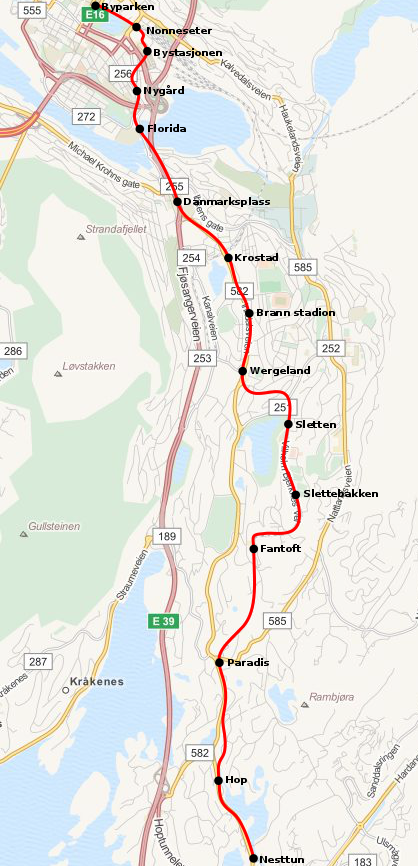
\includegraphics[width=.4\textwidth]{maps/Bergen_Karte.png}
  \caption{Streckenverlauf des neuen Straßenbahnabschnittes}
\end{wrapfigure}

Bergen ist eine etwa 270.000 Einwohner zählende Stadt in der Norwegischen
Provinz Hordaland.  und um Bergen befindet sich hügeliges, wetestgehend
unbewohntes Gelände. Bereits von 1897 bis 1966 verfügte Bergen über eine
elektrische Straßenbahn.

Bergen hat 2010 eine Stadtbahn von Byparken (Innenstadt) nach Nestun
eingerichtet. Die Strecke hat eine Länge von 9.8\,km, von denen 2.63\,km in 4
Tunneln liegen (Fageråstunnel (663\,m), Slettebakkstunnel (412\,m), Fantofttunnel
(1107\,m), Tveiteråstunnel (443\,m)). Die gesamte Strecke ist 2-gleisig ausgebaut
und verfügt über vereinfachte Zugsicherungs- und Signaltechnik mit
Vorrangschaltung gegenüber dem Straßenverkehr.

Die Strecke wurde von Januar 2008 bis Sommer 2010 errichtet. Etwa 5,9 km der
Strecke liegen gebündelt mit Straßen, jedoch auf eigenem Bahnkörper als
Rasengleis bzw. befahrbar für Rettungsfahrzeuge. Die restlichen 3,9 km sind
S-Bahn-ähnlich angelegt und beinhalten auch die vier Tunnel. Der minimale Radius
der Strecken beträgt 25 m, der maximale Neigungskoeffizient liegt bei 6\%.

Die Stadtbahn ist Teil des 500 Mio. Euro umfassenden \emph{Bergen-Programm für
Umwelt, Entwicklung und Verkehr}, welches von 2002 bis 2012 lief. Bis 2015 sind
hier weitere 143 Mio. Euro eingeplant, unter anderem für eine Erweiterung des
neuen Stadtbahnnetzes.

Die Gesamtkosten für das Projekt wurden auf 140 Mio. Euro projektiert, von denen
etwa 12 x 2,5 Mio. Euro für Fahrzeuge abzuziehen sind. Damit ergeben sich
Baukosten von ca. 110 Mio. Euro.

Seit Januar 2011 wird an der ersten Verlängerung nach Lagunen (3,6 km)
gebaut. Sie wurde am 21. Juni 2013 eröffnet.

Der dritte Bauabschnitt bis zum Flughafen soll im August 2013 begonnen und bis
2015 fertiggestellt werden. Er weist eine Länge von 6,5 km auf.

\section{Århus}

Århus ist die mit etwa 320.000 Einwohnern zweitgrößte Stadt in Dänemark. Für 2016
plant man, in Århus ein Stadtbahnnetz einzurichten, welches die Stadt und das
Umland verbinden soll.

Die geplante Neubaustreckenlänge umfasst 12,0 km. Diese werden auf eigenem
Bahnkörper, jedoch mit der Straße gebündelt ausgeführt. Die gesamte Strecke wird
zweigleisig ausgeführt.

Zur Erschließung des Umlandes wird eine etwa 95 km lange Eisenbahnstrecke für
den Betrieb mit Tram-Train-Fahrzeugen (Stadtbahnwagen) angepasst. Tunnelneu-
oder -umbauten sind nicht notwendig.

Die Kosten für den Straßenbahnabschnitt werden mit 500 Mio. Kronen angegeben,
was etwa 65 Mio.  Euro entspricht.

\section{Toulouse}

Wie viele französische Städte hatte auch Toulouse früher schon einmal ein Straßenbahnnetz, das jedoch bis 1957 komplett eingestellt wurde \cite{tlsesv}.
Es folgte eine Zeit der ausschließlichen Orientierung auf den motorisierten Individualverkehr, ÖPNV gab es nur in Form von Bussen.
Im Jahr 1993 wurde schließlich eine erste Metrolinie (Linie A) fertiggestellt und bis 2003 um drei Haltestellen erweitert, 2007 wurde eine zweite Linie eröffnet \cite{lafage}.
Um auch die Nachbargemeinden besser anbinden zu können, entschied man sich, als Ergänzung zur Metro ein Straßenbahnnetz aufzubauen. Die erste Strecke \textit{T1} ging 2010 in Betrieb, eine Verlängerung und ein Abzweig zum Flughafen sollen in den nächsten Monaten eröffnet werden.

\subsection*{Metrolinie B}

Die Linie wurde zwischen 2000 und 2007 erbaut, die Kosten betrugen \EUR{1150 Mio.}.
Wie schon die Linie A wird sie fahrerlos mit schiengeführten, aber gummibereiften \textit{VAL}-Zügen betrieben. So kann eine Geschwindigkeit von bis zu 80\,km/h und ein Zugabstand von 70 Sekunden erreicht werden \cite{lafage}.

Die Linie ist (mit Betriebsstrecke) 16,2\,km lang und hat 20 Haltestellen. Der öffentliche Teil ist vollständig unterirdisch, nur der Anschluss an die Abstellhalle ist teilweise oberirdisch \cite{lafage}.

\subsection*{Tramlinie T1}

\begin{wrapfigure}{r}{.41\textwidth}
  \includegraphics[width=.4\textwidth]{maps/Toulouse.png}
  \caption{Straßenbahnstrecke T1 in Toulouse}
\end{wrapfigure}

Die Strecke beginnt an der Metrostation \textit{Arènes}, wo Anschluss an die Metrolinie A und eine Vorortbahn besteht. Sie verläuft von dort nordwärts und erreicht nach etwa vier Kilometern den Vorort Blagnac, in dem auch der Flughafen und die Airbus-Werke liegen, beide werden von der Linie jedoch nicht direkt bedient, sie läuft stattdessen mittig durch die Gemeinde hindurch. Die Endhaltestelle, an der auch das Depot für die Bahnen gebaut wurde, liegt am Rande der Gemeinde Beauzelle \cite{lafage}.

Die Strecke kreuzt zwei Autobahnen, in einem Fall konnte eine existierende Straßenunterführung mitgenutzt werden, über die zweite Autobahn musste jedoch eine neue Brücke gebaut werden.


Baubeginn war 2007, die Eröffnung im Dezember 2010. Für die Baukosten gibt es unterschiedliche Angaben, laut Stadtverkehr \cite{tlsesv} sind es \EUR{157 Mio.}, laut einer Studie \EUR{212 Mio.}. Da mit letzterem Wert die Kosten weit über denen anderer Strecken liegen, vermuten wir, dass dort nicht direkt mit der Strecke zusammenhängende Kosten wie Betriebshöfe und dergleichen enthalten sind; wir arbeiten daher in der Auswertung mit der kleineren Zahl weiter.


\section{Dubai}

\begin{figure}[h]
  \begin{center}
    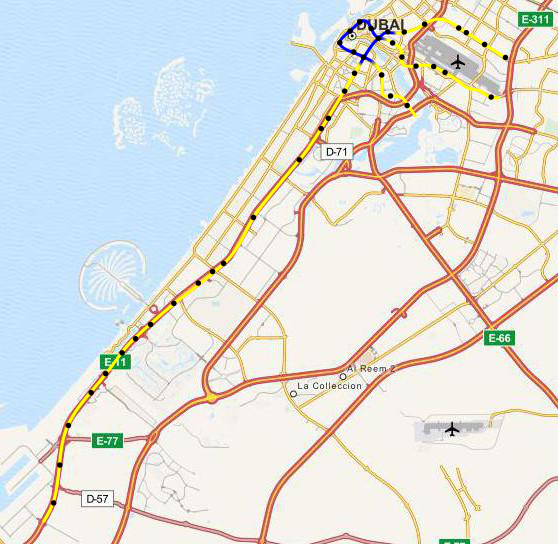
\includegraphics[width=0.8\textwidth]{maps/Dubai.png}
    \caption{Streckenverlauf der Metro Dubai}
  \end{center}
\end{figure}

Seit Oktober 2005 wird in Dubai ein komplett neues Metronetz
gebaut. Zuvor verfügte Dubai nur über ein dichtest preiswertes
Busliniennetz. Viele der Arbeitsmigranten sind auf den öffentlichen
Nahverkehr angewiesen, das sie sich kein Autoleisten können. Im
gegensatz dazu haben Familien mit mittleren bis hohen Einkommen meist
mehrer Fahrzeuge und nutzen daher den Nahverkehr nicht.

Bisher wurden auf zwei Linien 76\,km Streckennetz mit 47 Stationen
fertiggestellt. Davon verlaufen allerdings nur 12\,km im Zentrum
unterirdisch. Die restlichen 63\,km verlaufen als Hochbahn auf
Viaduktbauwerken. Die komplette Strecke ist zweigleisig ausgelegt und
verkehrt komplett führerlos. Sämtliche Stationen und Fahrzeuge sind
klimatisiert. \cite{hallodubai}

Während des Baus kam es immer wieder zu Problemen und
Kostensteigerungen. Bei der Eröffnung am 9.9.2009 um 9:09:09 Uhr
konnte nur ein Teilstück der ersten Linie eröffnet werden, da der
restliche Abschnitt noch in Bau war. \cite{tnDubaiMetro} Die komplette
Linie wurde erst im April des Folgejahres fertiggestellt. Durch die
Ölkriese sind die Kosten während des Baus explodiert. Nach
anfänglichen Planungen von 3.8\,Milliarden\,Euro mussten
Kostensteigerungen um 80\% auf 5.7\,Milliarden\,Euro hingenommen
werden. \cite{gnCosts}


Neben den bereits fertiggestellten Linien sind 2 weitere Linien mit
insgesammt 96\,km geplant. Der Baubeginn wurde allerdings durch die
Ölkriese auf unbestimmte Zeit verschoben. \cite{rtDubaiMetro} Eine
wieter Kuriosität ist, dass in einer Station der Metrolinie bis heute
keine Züge halten, da der entsprechende Stadtteil von Dubai sich durch
die Ölkriese noch nicht entwickelt hat.

\section{Brescia} 

\begin{figure}[h]
  \begin{center}
    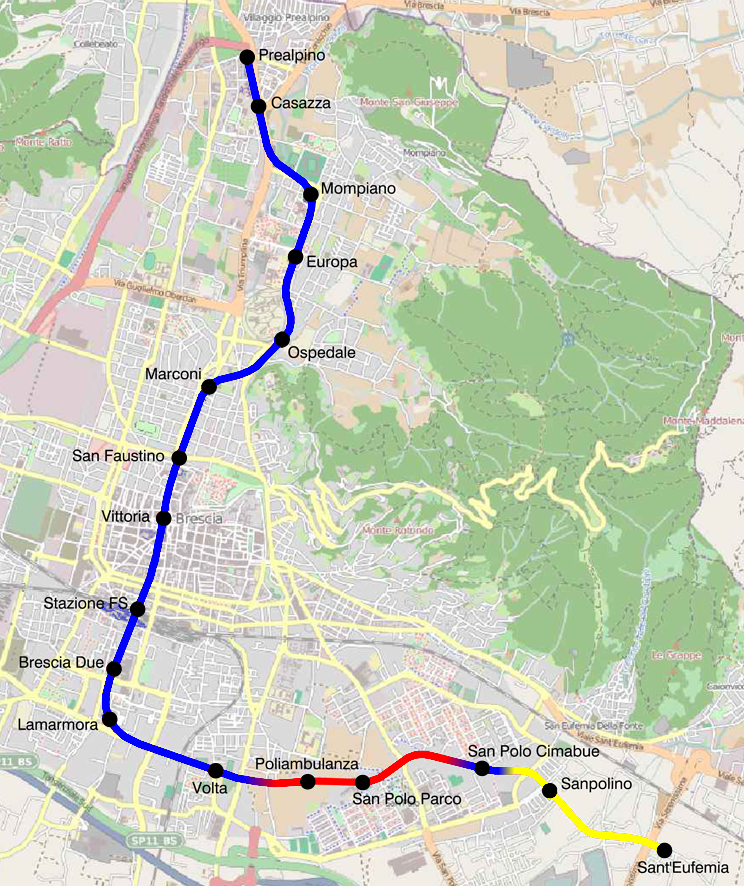
\includegraphics[width=0.8\textwidth]{maps/Brescia.png}
    \caption{Streckenverlauf der Metro in Brescia}
  \end{center}
\end{figure}

195 000 Einwohner hat Brescia. Für eine Stadt, die über eine 13.1\,km lange Metrobahn verfügt, ist das nicht viel. Dies ist sicherlich dem Stadtbahn-Finanzierungsgesetz zu verdanken, durch welches in Italien mitlerweile 60 Projekte mit \EUR{4341 Mio} gefördert wurden. Über 22 dieser Projekte, befinden sich mitlerweile im Betrieb. Die Gesammtkosten der 60 Projekte wurden mit \EUR{9629 Mio} beziffert. Am Beispiel Brescia wird allerding offenbar, das die tatsächlichen Kosten dieser Projekte weitaus höher sind. Die Metro in Brescia wurde am 11.06.2008 genemigt. Die Projektkosten wurden im Antrag mit \EUR{586 Mio} geschätzt.\cite{brescSv} Nach Fertigstellung und Inbetriebnahme werden die Kosten mittlerweile auf \EUR{935 Mio} beziffert, was einer Preisteigerung von etwa 60\% entspricht\cite{brescRai}.  

Vom Norden kommend, zieht sich die Metro Richtung Süden hin, unter der Stadt entlang. Unterhalb der Innenstadt und des Hauptbahnhofes ändert sich ihr Verlauf dann in einer weiten Kurve Richtung Osten. Auf dieser Tunnelstrecke liegen 12 der insgesammt 18 Stationen. Da sich in diesem Gebiet die Bebaung lichtet, verleuft die Metro die folgenden 1,7\,km ebenerdig übers teils offene Feld, weiter richtung Osten. In diesem Bereich liegen 2 weitere Stationen. Bevor die Linie auf den Lauf einer Straße trifft, der sie folgen wird, untertunnelt sie eine bebaute Straße, die sie kreuzt. Hier ligt die 13. unterirdische Station. In dem folgenden Streckenabschnitt läuft die Metro auf einem Viadukt, mittig einer großen Straße entlang. Dieser Abschnitt ist 1,7\,km lang und auf ihm liegen 4 Stationen.\cite{brescSts}


\begin{landscape}
\enlargethispage{2cm}
\begin{minipage}{\textwidth}
\section{Übersicht}
\include{results_table}
\end{minipage}
\end{landscape}


%%% Local Variables:
%%% mode: latex
%%% TeX-master: "main" %%% End:
